\Chapter{Szoftvereszközök numerikus számításokhoz}

    A numerikus számítások lényege, hogy valamilyen algoritmust végrehajtva
eljutunk a probléma megoldásához (vagy annak egy közelítéséhez), és ezt egy számítógépes
program segítségével tesszük. Ez a program lehet egy előre megírt
program csomag része, de akár írhatunk magunk is specifikus problémákra
saját programokat. Ezt megtehetjük akár egy olyan eltejedt általános célú
programozási nyelven, mint például a \textbf{C} vagy a \textbf{Java}, de
akár használhatunk egy ilyen feladatokra készített nyelvet vagy
programcsomagot is. A különbség a probléma megoldásának nehézségében és a hozzá szükséges időben rejlik,
hiszen az egyiket erre találták ki, előre definiálva vannak benne
szükséges függvények, konstansok, míg a másikban alapjaitól fel kell
építeni szinte mindent. Szerencsére jópár, numerikus számításokhoz
használható szoftvercsomag és nyelv létezik
Ebben a fejezetben ezekről,
ezek előnyeiről és hátrányairól fogok írni, illetve a fejezet végén
szó esik majd a \textbf{Python} eszközkészletéről is.

\Section{Alapvető elvárások}

Először is beszéljünk az alapvető elvárásokról, amiket egy ilyen
nyelvvel vagy szoftvercsomaggal szemben megkövetelhetünk. Kezdjük a
programozhatósággal! Fontos, hogy tudjunk benne programokat írni, hogy
speciális feladatokat tudjunk vele megoldani, esetlegesen új módszereket
tudjunk implementálni vagy csak egy módszer optimális implementációját
szeretnénk elkészíteni, és ne csak olyan problémákra adjon a
programcsomag megoldást amit előzetesen annak fejlesztői implementáltak.
A programozhatóság ebben a kontextusban elég, ha lekorlátozódik arra,
hogy itt matematikai problémák megoldására tudjunk programokat írni,
ezért nem feltétlenül kell általános nyelvnek lennie. Erre jó példa a
\textbf{Matlab}, amit mátrix műveletekhez optimalizáltak vagy az
\textbf{R}, ami egy statisztikai programcsomag. Ellenpélda a
\textbf{Python}, mely egy általános célú nyelv de a \texttt{NumPy} \cite{numpy} és
\texttt{SciPy} \cite{scipy} csomag segítségével használhatunk numerikus problémák
megoldására.

A programozhatóság mellett fontos még a programozási nyelv milyensége.
Általában matematikusok, kutatók, mérnökök használják ezeket tudományos
vagy mérnöki célokra, illetve diákoknak tanítják a numerikus módszereket
ezekkel a programcsomagokkal. Ők itt csak felhasználók, és nem mindig
várható el a felhasználóktól, hogy a programozás minden szempontjával és
fortélyával tisztában legyenek, így egy viszonylag könnyen tanulható és
használható nyelv az, amire szükség van.
Ilyen célokra, lehetőleg
valamilyen egyszerűen megérthető praradigmára építsen, mint az objektum
orientáltság vagy a procedurális programozás, vagy néha elég lehet az
is, ha csak matematikai formában adjuk meg a megoldandó feladatot. A
programozási nyelvek, melyekről itt majd részletesebb is lesz szó, elég
könnyen tanulhatóak (kivétel talán a \textbf{Fortran} ami egy régi,
nehezebben kezelhető nyelv, illetve a \textbf{Wolfram Matematica} eddig
említettektől teljesen eltérő szimbolikus nyelve). Ellenben a
\textbf{WolframAlpha} képes matematikai formában megadott problémákat is
megoldani.

Fontos még ezeken felül, hogy a programokat fájlokba tudjuk menteni és
ezáltal hordozhatóvá tenni őket, és ez nem csak a programok
forráskódjaira legyen igaz, hanem az eredményekre is. Szükséges az, hogy
el lehessen menteni a kapott eredményeket, adatokat későbbi
felhasználás, publikálás illetve áttanulmányozás érdekében. Az érem
másik oldala legalább annyira hasznos és fontos, be is kell tudni
olvasni az adatokat különböző adastruktúrákból, különböző formátumú
fájlokból, ezért szükséges a népszerűbb adatfájl formátumok támogatása,
mint például a CSV, JSON, XML vagy csak egy sima szöveges (\texttt{.txt}) fájl.

Az adatok mentése mellett a megjelenítésük is fontos lehet, hiszen az
emberek nagy része a grafikus ábrákból egyszerűbben le tudja olvasni az
adatokat, ezért szükséges, hogy a program csomag valamilyen módon tudjon
ábrákat készíteni. A programokat és módszereket nem csak megírni,
menteni és reprezentálni kell, hanem dokumentálni is azokat, ezért
szükséges hogy az adott nyelvnek és csomagnak ezt támogatnia kell. Egy
nagyon jó példa erre a \textbf{Python}, amivel használhatjuk a a
\texttt{Jupyter} munkafüzetet melyben a dokumentum cellákból épül fel, és
a cellákban egyszerre tudunk programozni és dokumentálni is.

A teljesítmény egy nagyon triviális követelmény, de egy nagyon fontos
tényező is, bár nagyon nagy adatokhoz szükséges egy erős hardver, de
szükséges az is, hogy gyengébb hardveren is futtatható legyen a kód
viszonylag jó futási idővel. Erre a problémára egy megoldás még a cloud
(felhő) amihez egy viszonylag gyors internet kapcsolat elég. Egyszerűen
működik, elküldjük a bemenő adatokat és a programot majd visszakapjuk az
eredményt, bár fontos megjegyezni, hogy ez érzékeny adatok esetén ez nem
lehet megoldás, hiszen a szerver üzemeltetői láthatják ezeket.

Egy utolsó, de nem elhanyagolható tényező, a programcsomag és az általa
használt nyelv elterjedtsége is, hiszen használhatjuk a lehető
leggyorsabb nyelvet ha a világban rajtunk kívül csak még egy páran
használják, de a világ többi része egy másik elfogadott nyelvet használ,
és így nehéz az általunk használt nyelvvel elhelyezkedni, vagy az
adatainkat és programjainkat megosztani másokkal, hiszen nem fogják
érteni és nem tudják majd futtatni.

\Section{Elterjedt matematikai szoftverek}

A következő pontokban áttekintem, hogy melyek az elterjedtebb, matematikai számítások végrehajtásához használt szoftverek.

\SubSection{Fortran}

A Fortran egy általános célú programozási nyelv melyet az IBM
fejlesztett ki még az 1950-es években \cite{fortran}.
Napjainkban is használatos és még
napjainkban is fejlesztik. Aránylag nehezen tanulható nyelv ami több
programozási paradigmát is támogat köztük az objektum orientáltságot,
procedurális és generikus programozást is. A Fortran támogatja a fájlba
írást de kimondott különböző fájlformátumú fájlok létrehozását nem, így
ha olyan fájlba szeretnénk az adatainkat menteni, nekünk kell
gondoskodni a formai követelményekről (például: CSV esetén nekünk kell
az elválasztó jelet kiteni az adatok közé).

\begin{figure}[h!]
\centering
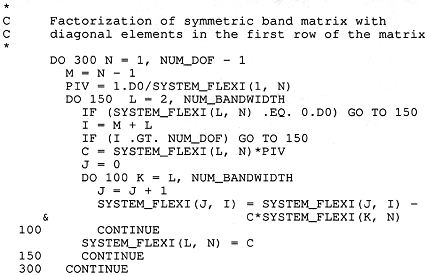
\includegraphics{img/FORTRAN_code_example.png}
\caption{Fortran forráskód részlet}
\label{fig:fortran}
\end{figure}

\Aref{fig:fortran}. ábrán egy Fortran forráskód részletet láthatunk. A kód a kötelező jellegű formázás miatt ugyan jól strukturált, viszont az alacsony szintű műveletek (mint például a \texttt{GO TO}) nehezítik a program működésének megértését.

\SubSection{Maple}\label{maple}

A \textbf{Maple} a Maplesoft által fejlesztett matematikai
szoftvercsomag, mely kombinál egy hatékony matematikai motort, mely a
számításokat végzi és egy könnyen használható felhasználói felületet,
ezáltal a használata egyszerű és gyors is tud lenni \cite{maple}.
A felhasználói
felület mellett parancssoros módban is képes működni, a saját nyelvét
használva. Scripteket is írhatunk melyet később megtudunk hívni.

\begin{figure}[h!]
\centering

\includegraphics{img/maple_logo.png}
\caption{A Maple szoftver logója}
\label{fig:maple-logo}
\end{figure}

\begin{figure}[h!]
\centering
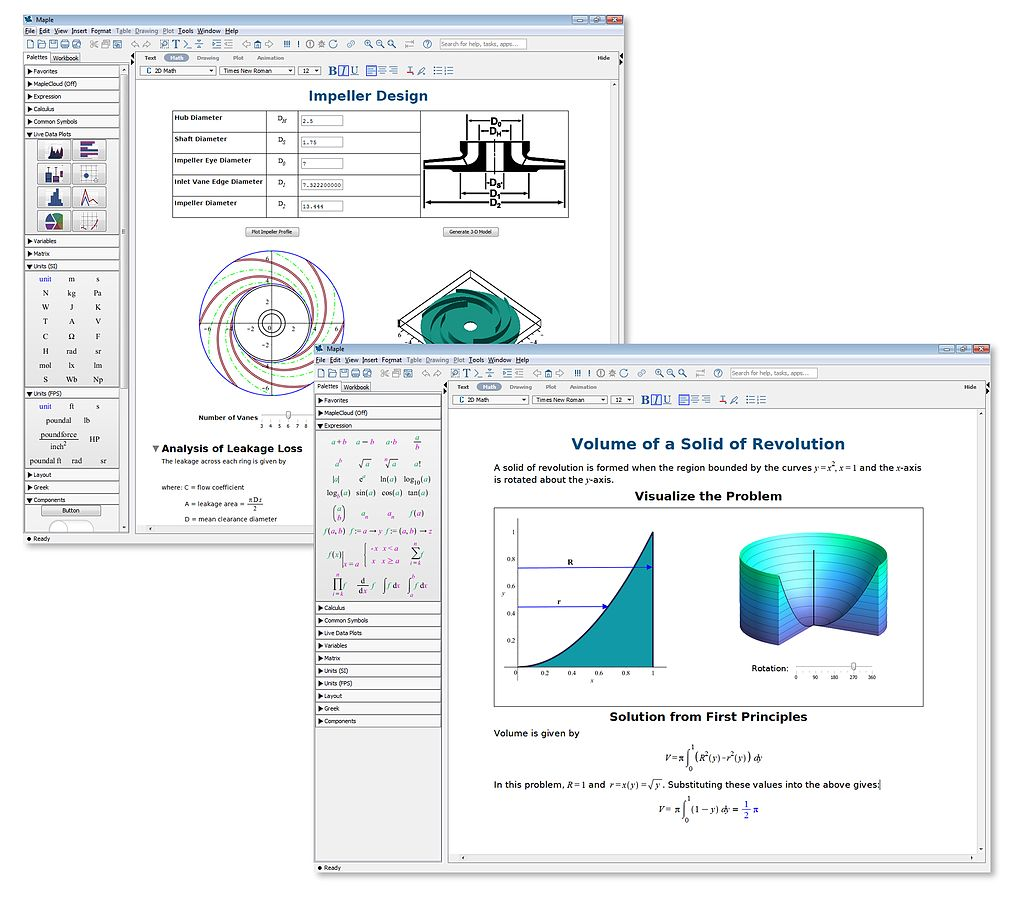
\includegraphics[width=\textwidth]{img/Maple_screenshots.jpg}
\caption[Maple]{Maple képernyőképek\footnotemark}
\label{fig:maple-screenshots}
\end{figure}

\Aref{fig:maple-logo}. ábrán láthatjuk a szoftver logóját, \aref{fig:maple-screenshots}. ábrán pedig néhány képernyőképet a grafikus felületéről.

A Maple-t mérnöki munkára és emellett rengeteg matematikai területen be
lehet vetni, például numerikus számításoknál, lineáris algebrában,
differenciál egyenleteknél. Nagyszerű az adatok vizualizálásában is. A
Maple nem ingyenes, licenszet kell hozzá vásárolni melynek ára elég
borsos, de itt is elérhető diák kedvezmény, mint a legtöbb ilyen
szoftvercsomag esetében, de 15 napig ingyenesen kipróbálhatja bárki.

Egyik előnye, hogy képes kommunikálni bizonyos szoftverekkel, mint a
Microsoft Excel, néhány CAD szoftver, SQLite adatbázisokkal, és az újabb
Matlab verziókkal is, ezzel könnyítve a munkát. Képes az ismertebb
adattárolásra használt fájlokba menteni és betölteni is, mint CSV, XLS.
Elérhető Microsoft Windowsra, Linuxra és Apple MacOS-re.

\footnotetext{forrás: \url{https://en.wikipedia.org/wiki/Maple_(software)}}

\SubSection{MATLAB}

A \textbf{Matlab} a MathWorks programcsomagja és programozási nyelve is
egyben, egy nagyon elterjedt nyelv a világon és számos helyen használják
különböző célokra mint: numerikus számítások, robotika, adat elemzés,
gépi tanulás, jel feldolgozás, kockázat elemzés, és irányító rendszerek \cite{matlab}.

\begin{figure}[h!]
\centering
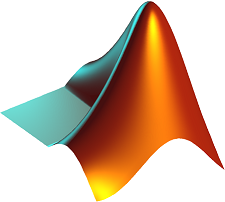
\includegraphics{img/Matlab_Logo.png}
\caption{A MATLAB szoftver logója}
\label{fig:matlab-logo}
\end{figure}

\begin{figure}[h!]
\centering
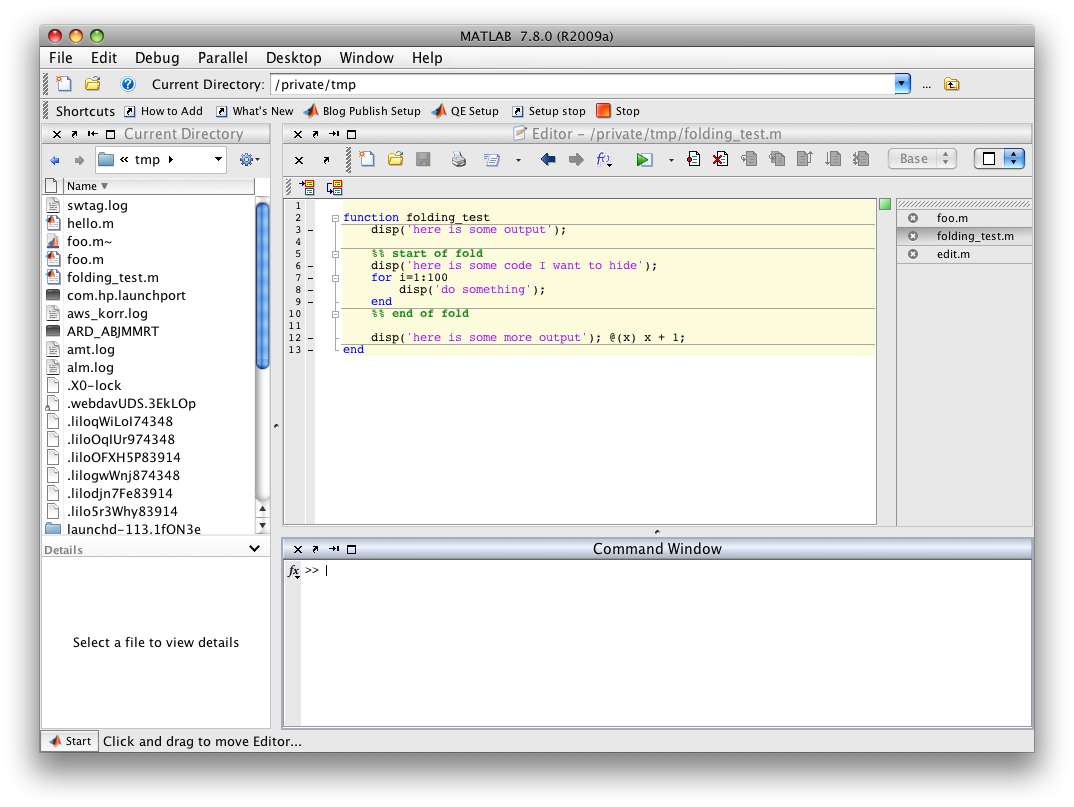
\includegraphics[width=\textwidth]{img/matlab_screenshots.png}
\caption[Matlab]{Képernyőkép a MATLAB grafikus felületéről\footnotemark}
\label{fig:matlab-screenshots}
\end{figure}

\Aref{fig:matlab-logo}. és \aref{fig:matlab-screenshots}. ábrákon láthatjuk a szoftver logóját és néhány képernyőképet.

Elsődlegesen mátrix műveletekre és numerikus számításokra készült,
ezáltal nagyon jól kezelei a mátrixokat és vektorokat.
Képes több szálon dolgozni és
támogatja a procedurális és objektum orientált programozási paradigmákat
is. A Matlab kódokat is menthetjük fájlba, ezáltal tudjuk tárolni,
publikálni (kiterjesztése: \texttt{.m}). Elérhető Microsoft Windows, Linux és
Apple MacOS operációsrendszerű gépekre. A Matlab nem egy ingyenes
szoftver meg kell vásárolni, de van lehetőségünk ingyenesen kipróbálni
illetve van kedvezmény diákok számára. A Matlab is képes importálni és
exportálni az adatokat a leginkább használt fájltípusokból.

% https://blogs.mathworks.com/community/2009/06/29/what-does-your-matlab-desktop-look-like-again

\footnotetext{forrás: \url{https://blogs.mathworks.com/community/2009/06/29}}

\SubSection{Python, NumPy és Matplotlib}

Ahogy a bevezető részben már említettem, a Python egy nagyon magas
szintű, platform független, általános programozási nyelv ami a világon
jelen pillanatban a 3. legnépszerűbb \cite{tiobe}
ebből adódóan nagyon elterjedt.
(A programozási nyelv logója \aref{fig:python-logo}. ábrán látható.)

\begin{figure}
\centering

\includegraphics[width=\textwidth]{img/python-logo.png}
\caption{A Python programozási nyelv logója \cite{python}}
\label{fig:python-logo}
\end{figure}

Nagyon nagy előnye a könnyű tanulhatósága és olvasható szintaktikája,
sokoldalúsága és bővíthetősége. Ezen tulajdonságai miatt rengeteg
területen alkalmazzák.

\begin{figure}
\centering
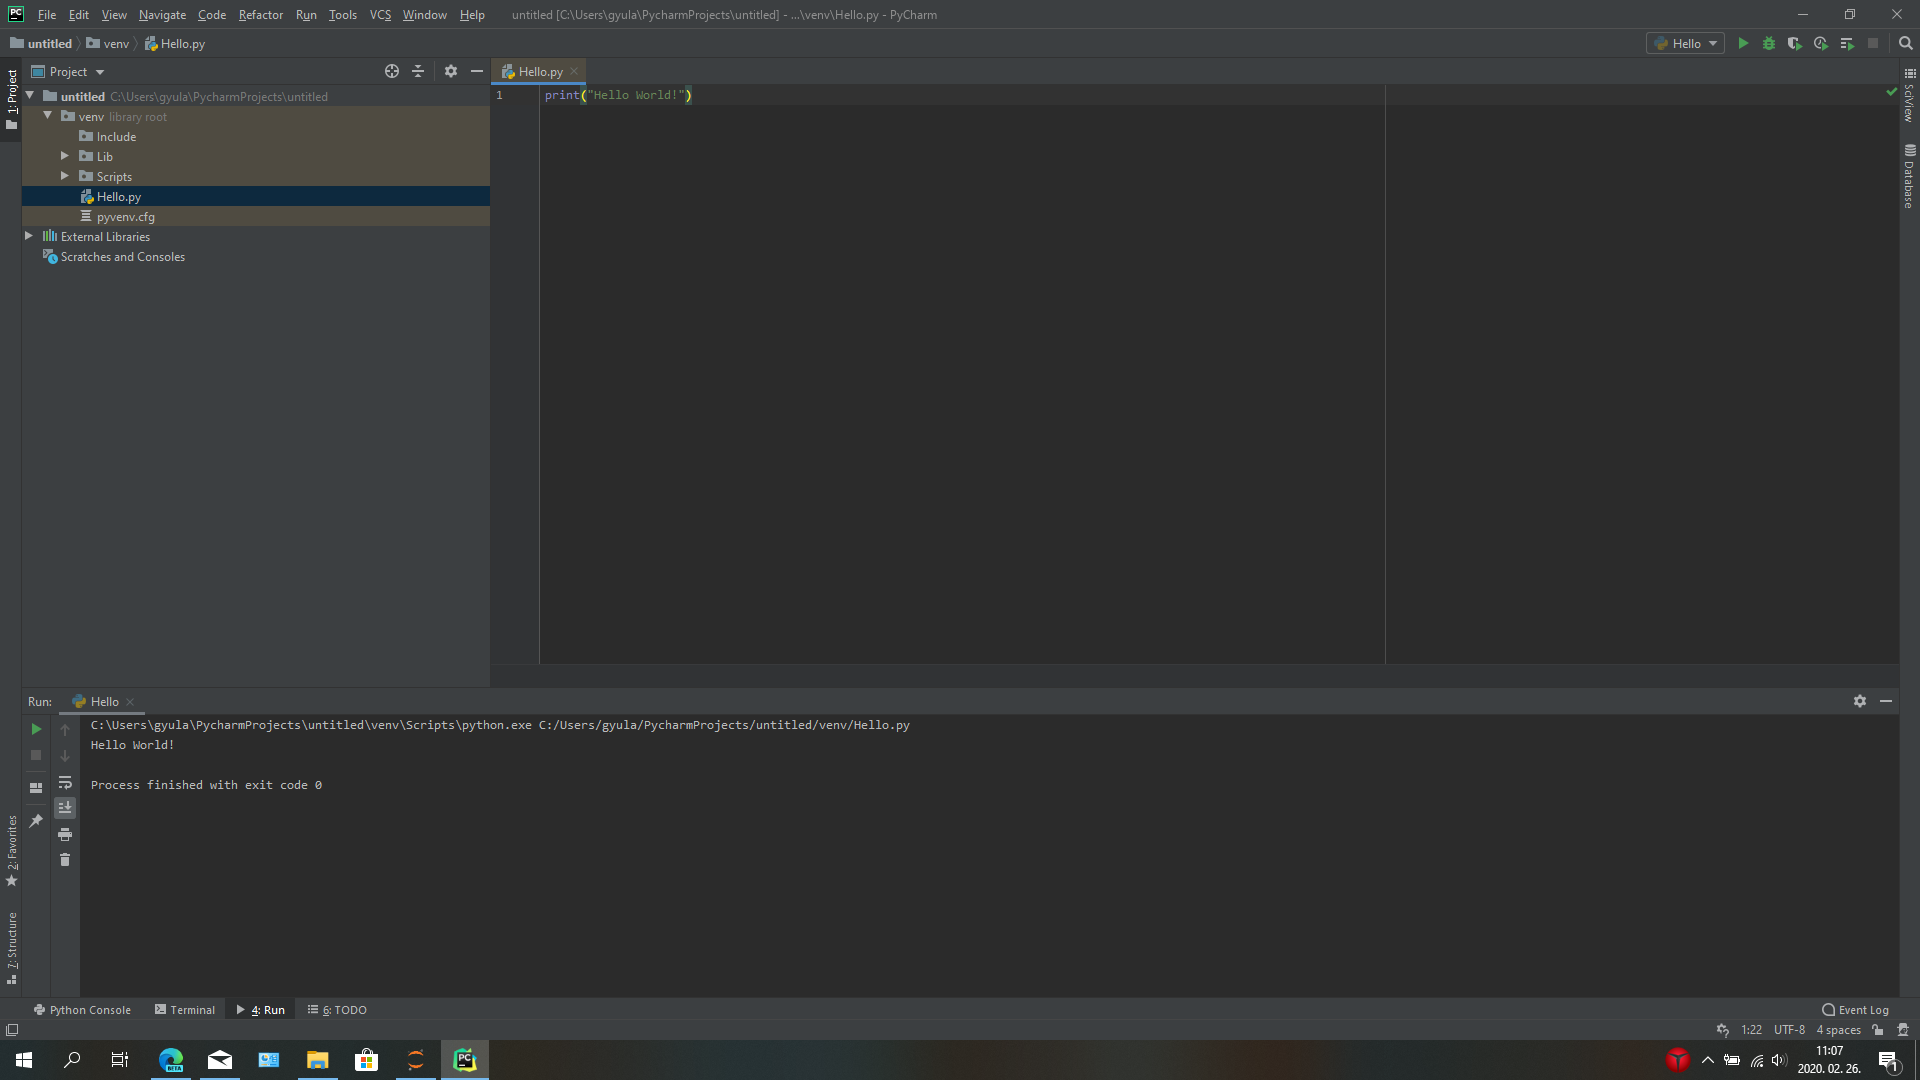
\includegraphics[width=\textwidth]{img/Python_screenshot.png}
\caption{Képernyőkép a PyCharm fejlesztőkörnyezetről}
\label{fig:pycharm}
\end{figure}

\begin{figure}
\centering
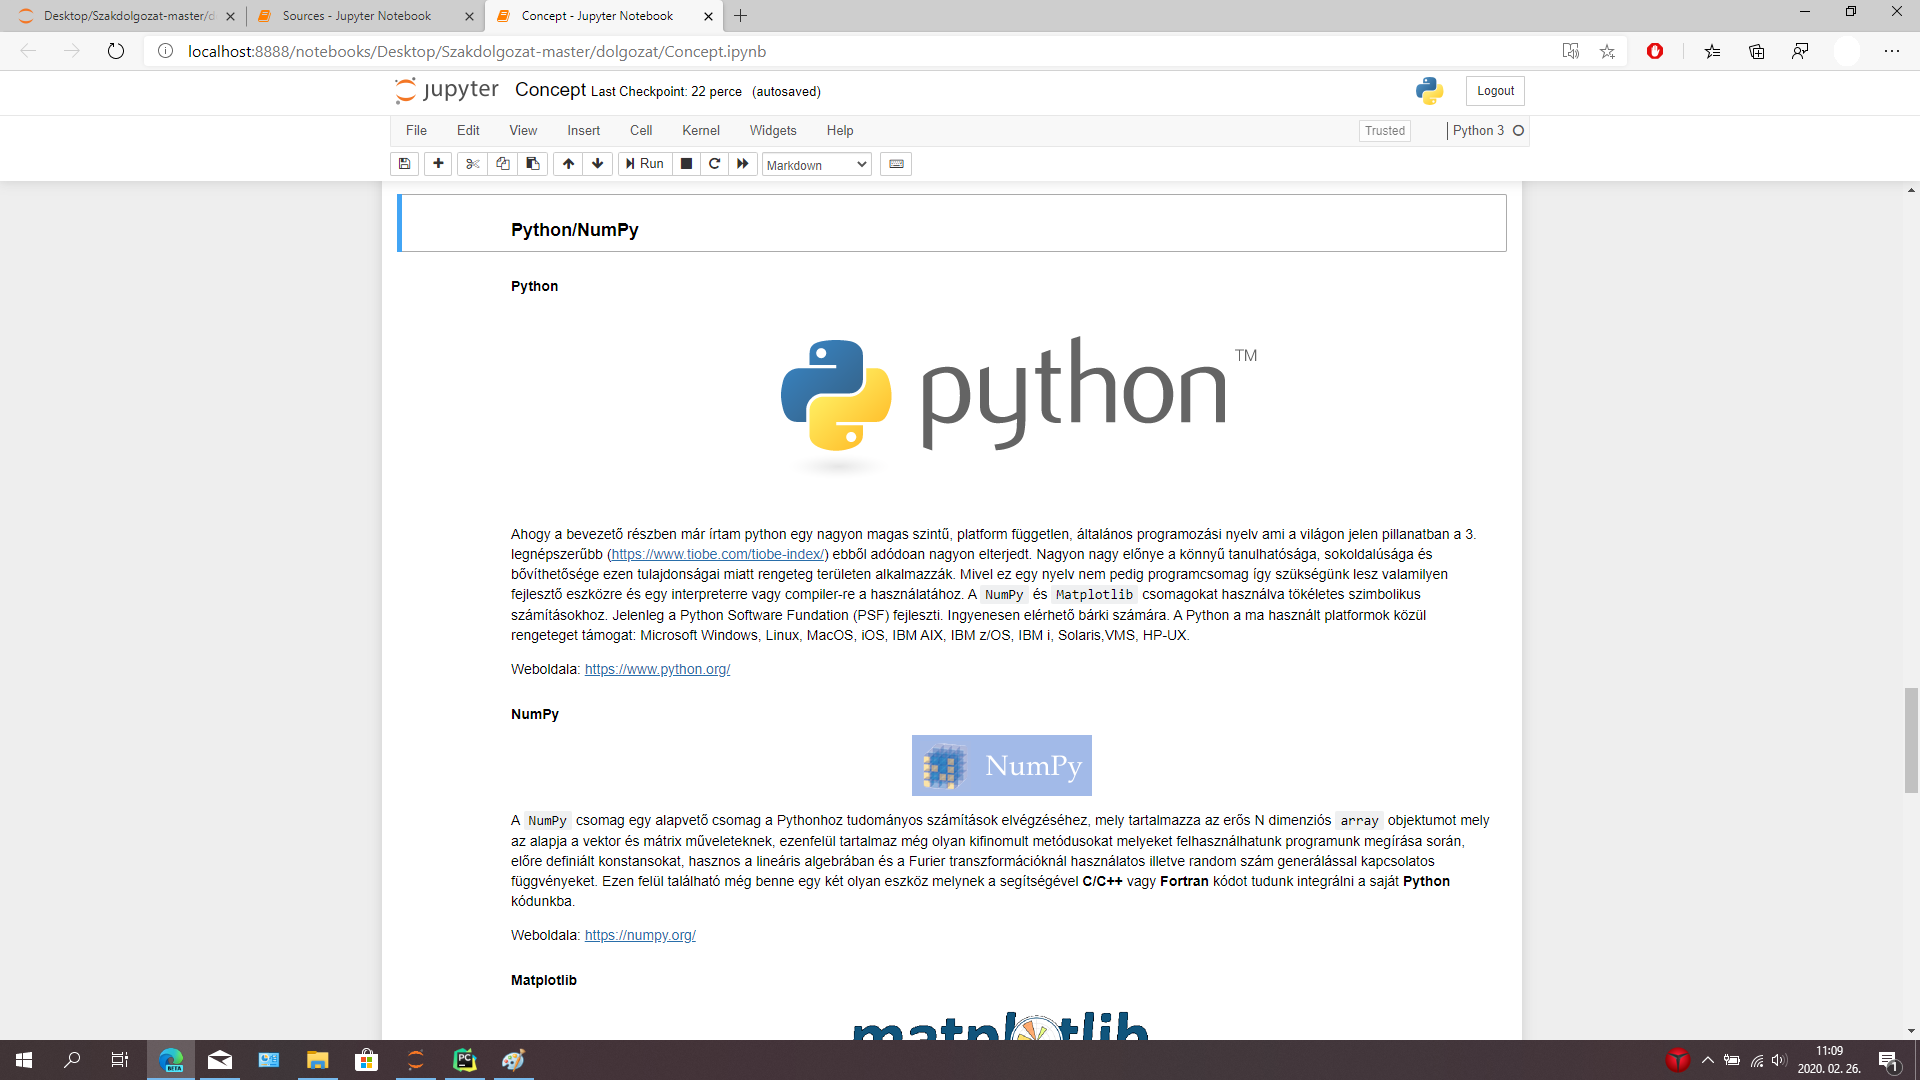
\includegraphics[width=\textwidth]{img/Jupyter_screenshot.png}
\caption{Képernyőkép egy Jupyter munkafüzetről}
\label{fig:jupyter}
\end{figure}

Mivel ez egy nyelv, nem pedig programcsomag így
szükségünk lesz valamilyen fejlesztő eszközre és egy interpreterre (vagy
compiler-re) a használatához.
Fejlesztőeszközök közül a PyCharm \cite{pycharm} (\ref{fig:pycharm}. ábra) és a Jupyter \cite{jupyter} (\ref{fig:jupyter}. ábra) az elterjedtebb eszközök.

A \texttt{NumPy}, \texttt{SymPy},
\texttt{SciPy} és \texttt{Matplotlib} csomagokat használva tökéletes
numerikus és szimbólikus számításokhoz. Jelenleg a Python Software
Fundation (PSF) fejleszti. Ingyenesen elérhető bárki számára. A Python a
ma használt platformok közül rengeteget támogat: Microsoft Windows,
Linux, MacOS, iOS, IBM AIX, IBM z/OS, IBM i, Solaris, VMS, HP-UX, mint
ahogy rengeteg fájltípust is támogat, adat export és adat importálás
szempontjából is.

A \texttt{NumPy} csomag egy alapvető csomag a Python-hoz tudományos
számítások elvégzéséhez, mely tartalmazza az erős $N$-dimenziós
\texttt{array} objektumot, mely az alapja a vektor és mátrix
műveleteknek, ezenfelül tartalmaz még olyan kifinomult metódusokat
melyeket felhasználhatunk programunk megírása során, előre definiált
konstansokat, hasznos a lineáris algebrában és a Fourier
transzformációknál, illetve véletlenszám generálással kapcsolatos
függvények is elérhetők benne \cite{numpy}. Ezen felül található még két olyan eszköz
melynek a segítségével \textbf{C/C++} vagy \textbf{Fortran} kódot tudunk
integrálni a saját \textbf{Python} kódunkba.

A \texttt{Matplotlib} csomag segítségével tudjuk vizualizálni az
általunk használt adatokat vagy általunk kiszámított adatokat \cite{matplotlib}. 2D-s
grafikonokat és ábrákat készíthetünk a segítségével. Az ábrákat tudjuk
menteni is külön fájlba, a Cairo segítségével akár vektorgrafikusan is.

\SubSection{GNU R}

A \textbf{GNU R} egy ingyenes szoftvercsomag, melyet elsődlegesen a
statisztikai számítások során alkalmaznak \cite{gnur}.
Az \textbf{R} nem csak egy
programcsomag hanem egy programozási nyelv is egyben.

\begin{figure}[h!]
\centering

\includegraphics{img/R_logo.png}
\caption{A GNU R logója}
\label{fig:r-logo}
\end{figure}

\begin{figure}[h!]
\centering
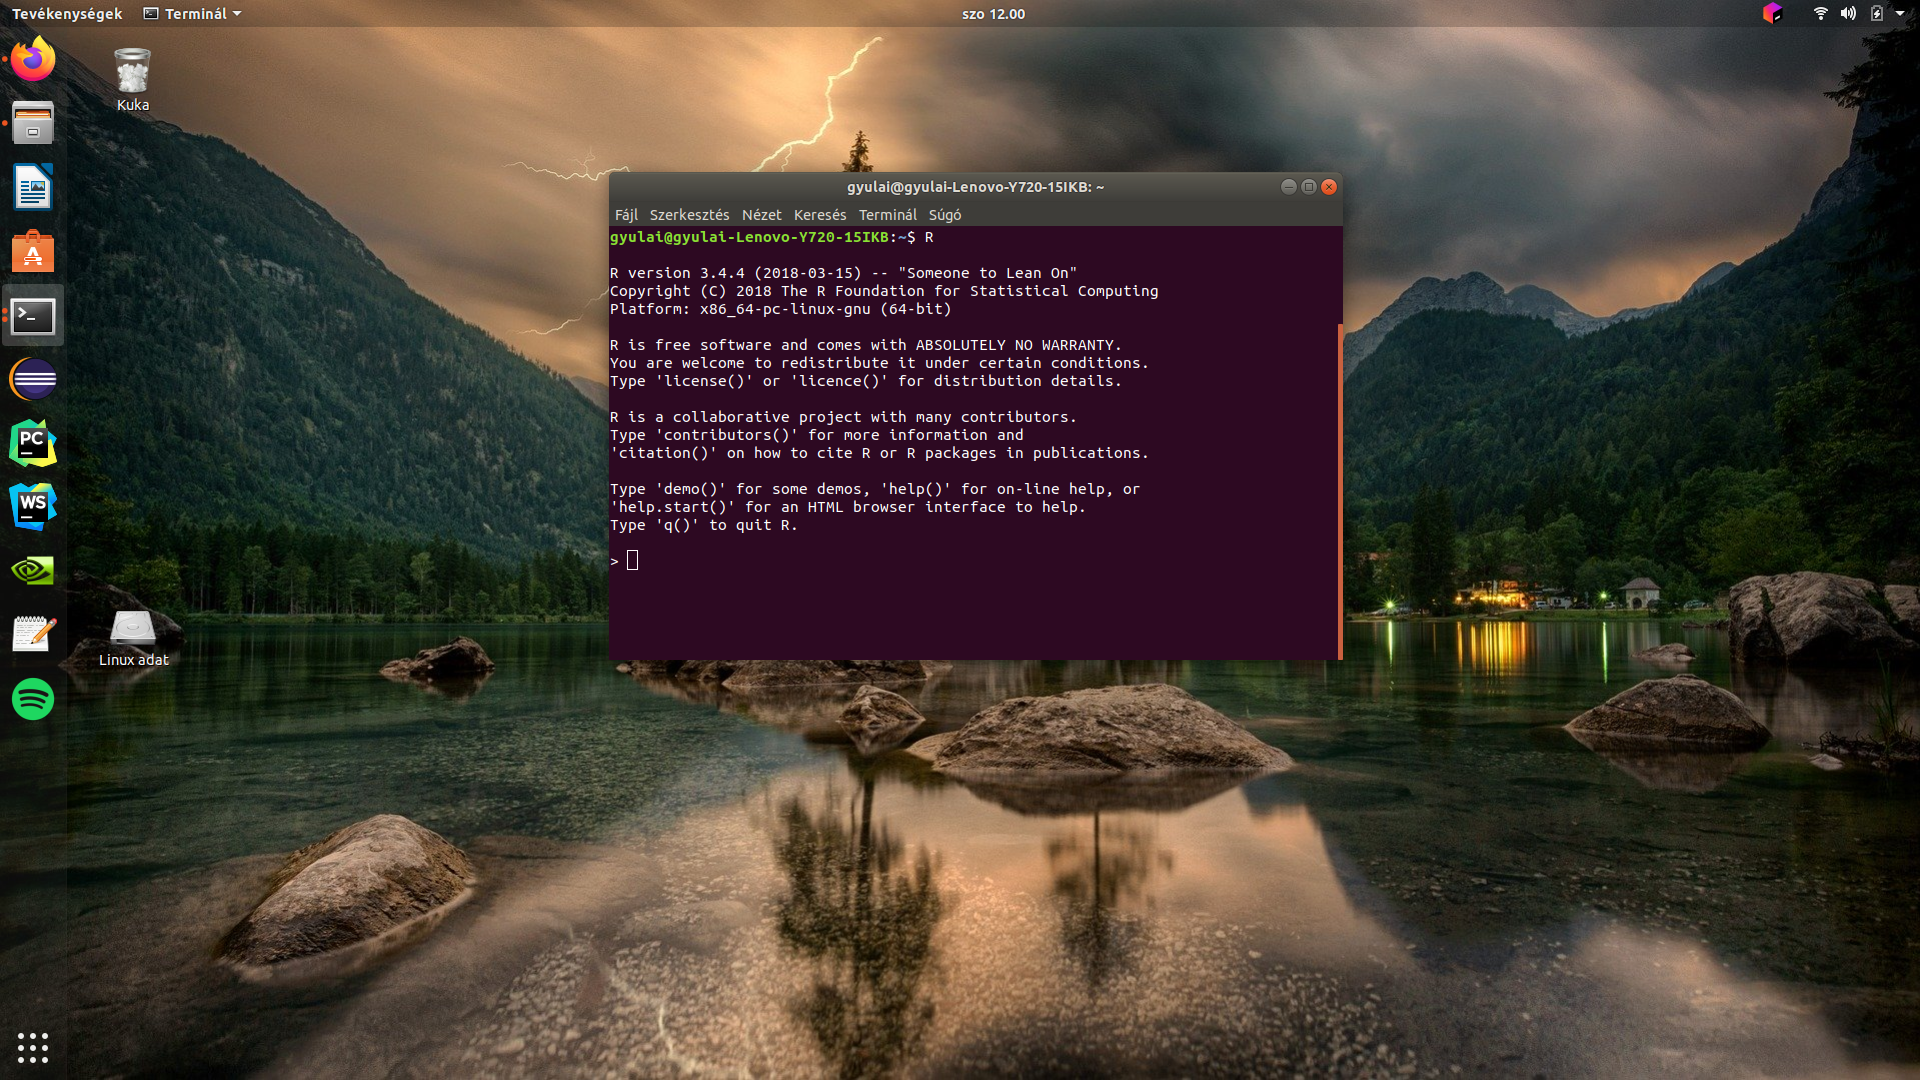
\includegraphics[width=\textwidth]{img/R_screen.png}
\caption{Képernyőkép a GNU R használatáról}
\label{fig:r-screenshot}
\end{figure}

A programcsomag logóját és egy képernyőképet a program használatáról \aref{fig:r-logo} és \aref{fig:r-screenshot}. ábrákon tekinthetünk meg.

Az R-t, ahogy már
említettem statisztikai problémák megoldásánál érdemes használni, de a
nyelv egy nagy előnye, hogy nyílt forráskódú és ezáltal nagyon sok
csomag készült hozzá és ez kibővíti a képességeit több irányba is. Az R
elérhető Microsoft Windowsra, Linuxra, és Apple MacOS-re is. Az R is
képes importálni és exportálni az adatokat a leginkább használt
fájltípusokból, mint a CSV vagy XLS.

\SubSection{Wolfram: Mathematica, Wolfram
Alpha}

\begin{figure}
\centering
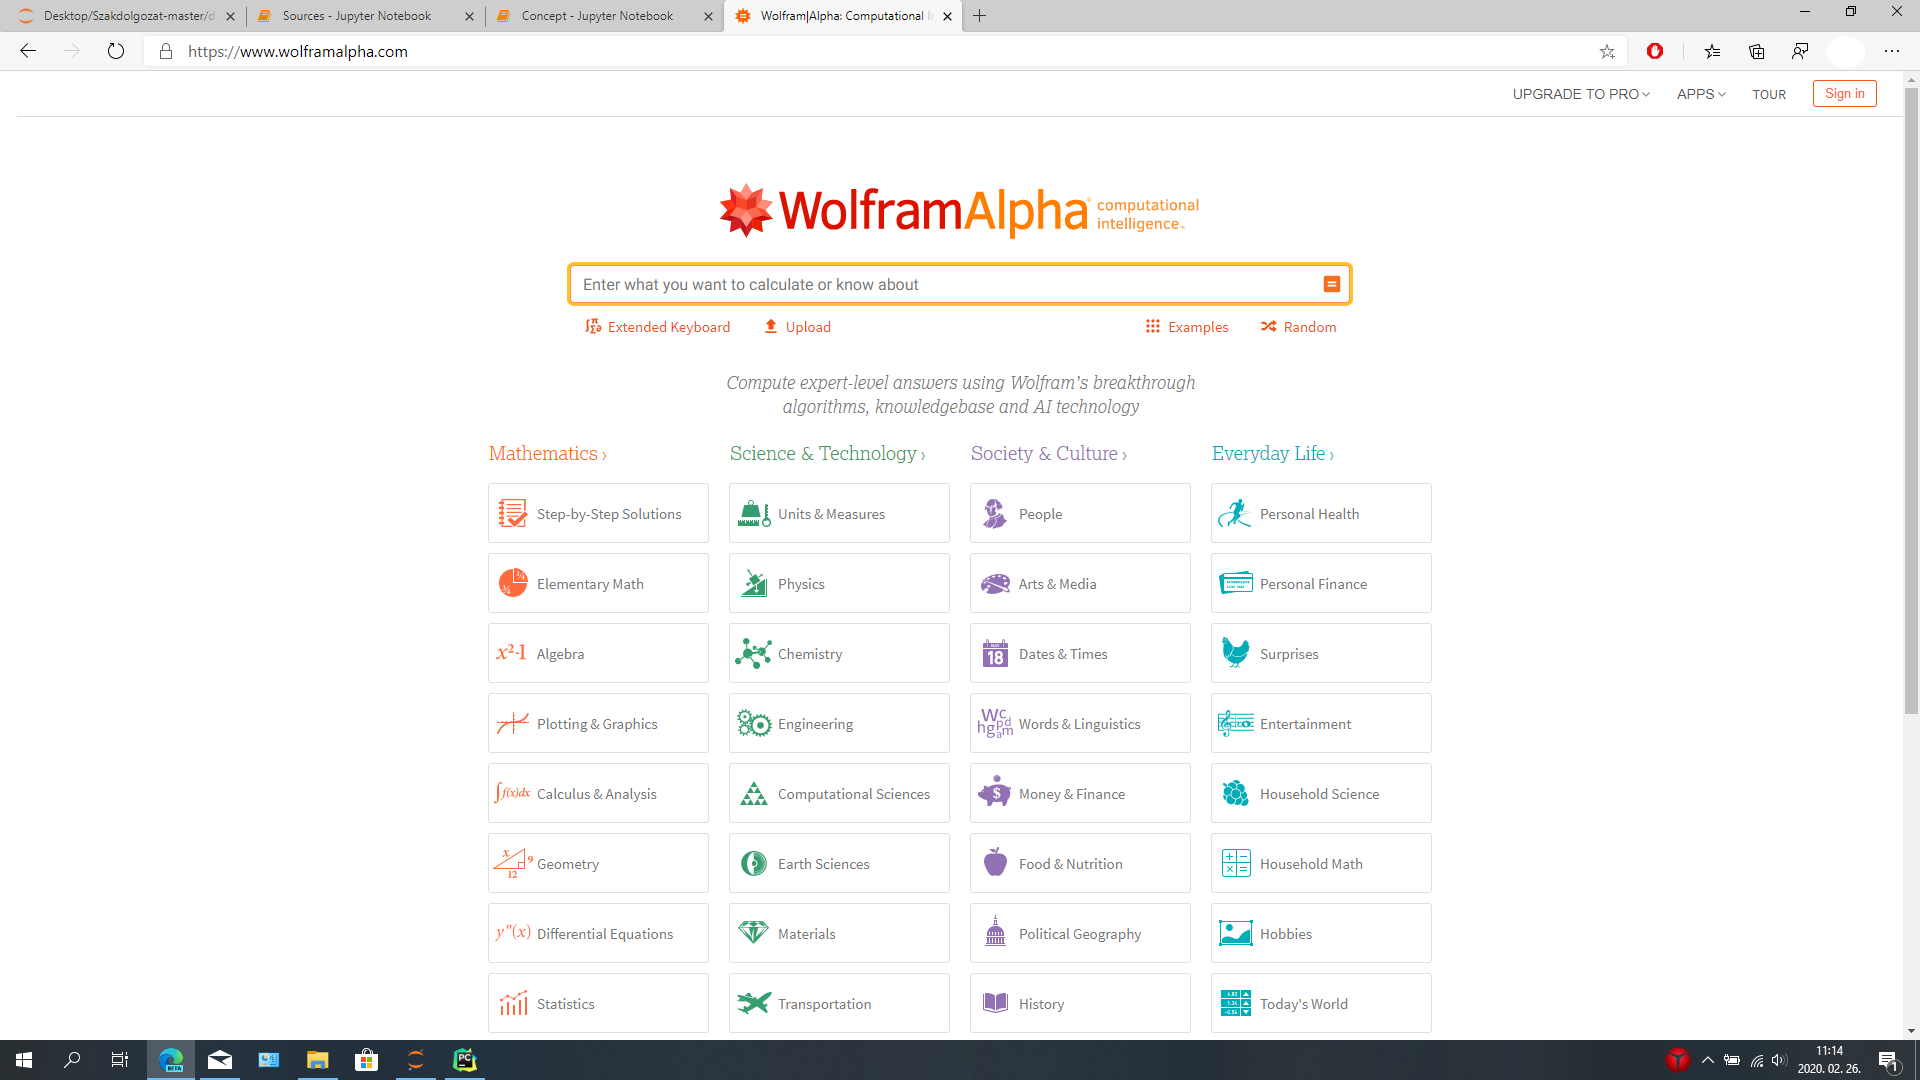
\includegraphics[width=\textwidth]{img/alpha_screen.png}
\caption{Egy képernyőkép a Wolfram Alpha weboldaláról}
\label{fig:wolfram-alpha}
\end{figure}

A Wolfram Alpha nem is igazán egy szoftvercsomag inkább egy probléma
megoldó szoftver, melyet a Wolfram fejleszt és mely ötvözi a természetes
nyelv feldolgozást, az adatbányászatot és a dinamikus programozást,
ezáltal talál a megadott problémára megoldást.
(\Aref{fig:wolfram-alpha}. ábrán láthatjuk, hogy hogy néz ki a szoftver használatát biztosító weboldal.)

Az Alpha mögött óriási
adatbázis van. Létezik ingyenes megvalósítása mely elérhető a
weboldalán, illetve van egy Wolfram Alpha Pro elnevezésű változata is,
mely többet nyújt de fizetni kell érte. Az Alpha a fejlesztőknek
rengeteg API-t (\emph{Application programming Interface}, magyarul
alkalmazásprogramozási interfész) nyújt melynek egy része ingyenes, egy
részéért viszont szintén fizetni kell.

A Matematica szintén a Wolfram által fejlesztett matematikai
programcsomag, a Matlab-hoz illetve a Maple-höz hasonlóan rengeteg
területet lefed
\cite{wolfram}.
A Wolfram nevezetű szimbólikus programozási nyelvet
használja, mely az eddigiektől nagyon eltérő. A programcsomag szintén
nem ingyenes. Elérhető Microsoft Windowsra, Linuxra és Apple MacOS-re,
és itt is találunk diák kedvezményt. Ha nem szeretnénk megvenni a teljes
csomagot, vagy nincs elég erős számítógépünk hozzá, akkor elérhető a
Matematica Cloud amire elő lehet fizetni egy évre, és csak egy böngésző
és internet kapcsolat szükséges hozzá. Az Alpha és a Matematica is
támogatja az adatok importálását és exportálását népszerű formátumú
fájlokba.

\Section{Python eszközkészlet}

    A szakdolgozatban a Python nyelvet fogom használni és azon belül is
nagyrészt a Jupyter munkafüzetben dolgozom. Ahhoz, hogy Python-ban
tudjunk dolgozni szükségünk van egy Python értelmezőre. Ez értelmezi a
kódot és hajtja azt végre. Több fajta Python interpreter létezik. A
legelterjedtebb a CPython mely C-ben és Python-ban íródott, ez a
referencia interpreter és ebből indul ki a többi interpreter is. Van
interpreter mely engedi hogy Java nyelvű kódot használjunk, és olyan is
mely a Python kódot lefordítja C vagy C++ nyelvű kóddá, vagy éppen olyan
is ami JavaScript-et vagy Java kódot varázsol a mi kis Python kódunkból.

Mivel Jupyter munkafüzetet használok, így használom az IPython nevezetű
shellt is \cite{ipython}.
Az IPhyton tartalmazza a Jupyter kernelét és támogatja különböző
interpreterek használatát. Itt most a referencia CPython interpretert
használom majd. Ezen felül támogatja az IPhyton az interaktív adat
vizualizációt, interaktív elemek beépítését a munkafüzetbe, valamint a
párhuzamosítást is ha szükség lenne rá, illetve támogat különböző GUI
toolkiteket is. Az Adatok vizualizációjáért a fent már említett
Matplotlib csomag lesz felelős.

Ahhoz, hogy programozzunk valamilyen nyelven, kell valamilyen szöveg
szerkeztő vagy IDE és ez a Pythonnal sincs másképp. Pythonhoz elérhető
több nagytudású IDE is, mint a Spyder, Jupyter, Pycharm.

Kezdjük a Jupyterrel! Ez egy open-source web-alkalmazás, mely olyan
dokumentumok létrehozását, szerkesztését, megosztását teszi lehetővé
melyben a programkódok lefuttathatóak, ezáltal olyan interaktív
dokumentumot készíthetünk melyben a programok bemutathatóak és a kapott
adatok könnyen vizualizálhatóak. A Jupyter több mint 40 programozási
nyelvet támogat.

Használhatjuk akár a Spyder-t is ami eg IDE kifejezetten Pythonhoz.
Főleg tudományos célú használatra készült, és mint a Jupyter az IPythont
használja. mint minden IDE-t könnyű telepíteni és elkezdeni vele
dolgozni. Az Anaconda platformon belül ingyenesen érhető el.

Harmadik fejlesztő eszközünk a Pycharm, amit a JetBrains fejleszt.
Létezik egy ingyenes Community Edition és egy megvásárolható
Professional Edition. A Professional Edition sokkal több funkciót
támogat a Community Edition-nel szemben, például a Jupyter notebookok
szerkeztését és megtekintését. A PyCharm azoknak kimondottan előnyös,
akik használtak már valamilyen másik JetBrains által fejlesztett IDE-t,
hiszen a megszokott kezelő felülettel fognak találkozni.
